% !TeX program = pdflatex
% !TeX encoding = UTF-8
%=======================================================================
%  GRIS-NOT-001  ·  Plantilla de notas rápidas para la memoria
%  Proyecto 00503 - Generator inspection robotic system · Mecanalisis
%  Identidad: GRIS-IDENTIDAD-001 v1.4
%-----------------------------------------------------------------------
%  CÓMO USARLA (en 3 pasos)
%
%   1. Copiá este archivo con el código de la nota:
%         memoria/notas/02489-00-MC007.tex
%      El número (###) es correlativo: mirá la última nota y sumá uno.
%
%   2. Completá los cuatro datos del bloque «DATOS DE LA NOTA».
%
%   3. Escribí:
%        · Resultados (obligatorio, siempre primero): lo que se sabe
%          ahora que antes no se sabía. Frases cortas, con números.
%        · El resto es libre. Usá los títulos que te sirvan, o ninguno.
%
%   Compilar:  pdflatex 02489-00-MC007.tex
%   En Overleaf: subí el .tex y logo-gris.pdf.
%
%  LOGO: se usa «logo-gris.pdf» (GRIS-LOGO-003, reducido) de esta carpeta
%  o de ../plantilla/. Si falta, se escribe «GRIS» como marcador.
%=======================================================================
\documentclass[11pt,a4paper]{article}

%=======================================================================
%  DATOS DE LA NOTA  ← lo único que hay que tocar arriba
%=======================================================================
\newcommand{\codigo}{02489-00-MC006}          % 02489-00-MC###
\newcommand{\titulo}{Forma y largo del flex del conector M12}
\newcommand{\autor}{Matías Gaviño}
\newcommand{\fecha}{28/09/2026}                    % o p. ej. {24/09/2026}

%=======================================================================
%  ESTILO  (no hace falta tocar nada de aquí hasta \begin{document})
%=======================================================================
\usepackage[T1]{fontenc}
\usepackage[utf8]{inputenc}
\usepackage[spanish,es-noshorthands,es-tabla]{babel}
\usepackage{lmodern}
\usepackage[a4paper,top=3.0cm,bottom=2.4cm,left=2.4cm,right=2.4cm,
            headheight=20pt,headsep=1.2cm,footskip=1.1cm]{geometry}
\usepackage{microtype}
\usepackage{xcolor}
\usepackage{graphicx}
\usepackage{booktabs}
\usepackage{array}
\usepackage{enumitem}
\usepackage{titlesec}
\usepackage{fancyhdr}
\usepackage{caption}
\usepackage{amsmath,amssymb}
\usepackage{float}
\usepackage[hidelinks]{hyperref}

% --- colores -----------------------------------------------------------
\definecolor{gris-naranja}{HTML}{FF7A00}   % naranja institucional
\definecolor{tinta}{HTML}{1E2328}
\definecolor{gris-medio}{HTML}{6B7280}
\definecolor{gris-linea}{HTML}{DADDE1}
\color{tinta}

\hypersetup{pdftitle={\codigo\ -- \titulo}, pdfauthor={\autor},
            colorlinks=true, linkcolor=tinta, urlcolor=tinta}

% --- logo ---------------------------------------------------------------
\graphicspath{{./}{../plantilla/}{plantilla/}{02489-00-MC006/figuras/}}
\newcommand{\logogris}{%
  \IfFileExists{logo-gris.pdf}
    {
\includegraphics[height=16pt]{logo-gris.pdf}}
    {\IfFileExists{../plantilla/logo-gris.pdf}
      {
\includegraphics[height=16pt]{../plantilla/logo-gris.pdf}}
      {{\fontsize{18}{18}\selectfont\bfseries\sffamily\color{gris-naranja}GRIS}}}}

% --- tipografía del cliente (código documental) --------------------------
% Geogrotesque no es libre; se usa Roboto Condensed Bold, que viene con
% TeX Live y Overleaf y tiene el mismo aire que el logo.
\newcommand{\fuentecliente}{\fontfamily{Roboto-TLF}\fontseries{bc}\selectfont}

% --- encabezado y pie ---------------------------------------------------
\pagestyle{fancy}
\fancyhf{}
\renewcommand{\headrulewidth}{0.4pt}
\renewcommand{\headrule}{\vspace{3pt}{\color{gris-linea}\hrule height \headrulewidth}}
\fancyhead[L]{\logogris}
\fancyhead[R]{{\fuentecliente\fontsize{12}{12}\selectfont\color{gris-medio}\codigo}}
\fancyfoot[R]{\footnotesize\color{gris-medio}\thepage}

% --- títulos numerados ----------------------------------------------------
\setcounter{secnumdepth}{2}
\titleformat{\section}{\large\bfseries}{\thesection}{0.8em}{}
\titleformat{\subsection}{\normalsize\bfseries}{\thesubsection}{0.8em}{}
\titlespacing*{\section}{0pt}{16pt}{5pt}
\titlespacing*{\subsection}{0pt}{11pt}{3pt}

% --- texto ------------------------------------------------------------------
\setlength{\parindent}{0pt}
\setlength{\parskip}{6pt}
\linespread{1.05}
\setlist{topsep=2pt, itemsep=2pt, parsep=0pt, leftmargin=1.2em}
\setlist[itemize]{label={\raisebox{0.15ex}{\small$\bullet$}}}
\captionsetup{font={small,color=gris-medio}, labelfont=bf, skip=5pt}
\renewcommand{\arraystretch}{1.25}

% --- cabecera de la nota ------------------------------------------------------
\newcommand{\cabecera}{%
  \thispagestyle{fancy}%
  {\fontsize{20}{24}\selectfont\bfseries\titulo\par}%
  \vspace{5pt}%
  {\small\color{gris-medio}\fecha\quad·\quad\autor\par}%
  \vspace{6pt}}

% --- ayudas opcionales --------------------------------------------------------
% \figura{archivo}{ancho}{pie}
\newcommand{\figura}[3]{%
  \begin{figure}[htbp]\centering
    \includegraphics[width=#2\linewidth]{#1}\caption{#3}
  \end{figure}}

%=======================================================================
\begin{document}
\cabecera

%-----------------------------------------------------------------------
%  RESULTADOS  (siempre primero, lo único obligatorio)
%  Qué se sabe ahora. Cada punto se entiende sin leer el resto.
%  Si hay un número, ponelo: «error < 2 mm», no «error bajo».
%-----------------------------------------------------------------------
\section{Resultados}
\textbf{El flex del conector M12 es una S en el plano de las placas, de 19,0~$\pm$~0,25~mm entre cantos
rígidos.} Une el canto de la placa del conector con el de una pestaña fija de la mainboard, separados
15,5~mm a lo largo de las placas; la pestaña queda 5~mm detrás de la línea del flex. Los números salen de la simulación
de la elástica (\texttt{flex\_omega/s\_layout.py}) y de \texttt{02489-00-MC006/calculo.py}.

\begin{table}[H]\centering\small
\begin{tabular}{l l l c}
\toprule
Requisito & Límite & Resultado (peor caso con tolerancias) & Cumple\\
\midrule
Radio interior en toda la carrera & $\geq$ 2,5~mm & 2,79~mm (2,84~mm con cotas nominales) & sí\\
Juego a la placa de cámara & $\geq$ 0,3~mm & 1,43~mm & sí\\
Carrera de la placa del conector & 12~mm & verificada con 12 y 12,5~mm & sí\\
Recto en cada transición rígido-flex & 1~mm & 1~mm & sí\\
Separación entre cantos (Z) & mínima & 15,5~mm & ---\\
\bottomrule
\end{tabular}
\end{table}

\begin{itemize}
  \item \textbf{Largo del flex: 19,0~$\pm$~0,25~mm.} Con 18,75~mm el juego a la placa de cámara baja a
        1,43~mm; con 19,25~mm el radio interior baja a 2,79~mm. Los dos extremos cumplen.
  \item \textbf{No acortar por debajo de 18,5~mm.} Con 18,25~mm el flex se tensa, apoya en la placa de
        cámara y el radio cae a 1,77~mm.
  \item \textbf{Para dibujar alcanzan tres arcos de R~3,5 unidos por rectas} (sección~\ref{sec:geometria}):
        21,5°, 83,5° y 62°, con rectas de 1,00 / 3,39 / 3,41 / 1,00~mm. Tiene el mismo largo y los
        mismos extremos que la forma simulada y se aparta de ella 0,11~mm como máximo.
  \item \textbf{La S tiene que quedar libre.} Apoyada contra una pared salta de forma en la carrera
        (\emph{snap-through}) y el radio cae de golpe.
  \item \textbf{Pendiente:} confirmar con una muestra el largo real entre cantos después del fresado y el
        comportamiento del flex con el cobre de las dos capas.
\end{itemize}

\section{Problema}
La placa del conector M12 tiene que retroceder 12~mm detrás del panel para montar el equipo y después
volver a su lugar. La mainboard, con su pestaña fija, no se mueve. El flex que une las dos placas absorbe
esa carrera en su propio plano, sin pasarse del radio admisible y sin tocar la placa de la cámara, que
queda al lado. Lo que se minimiza es la separación entre cantos (Z), no el largo del flex.

\begin{figure}[H]\centering
  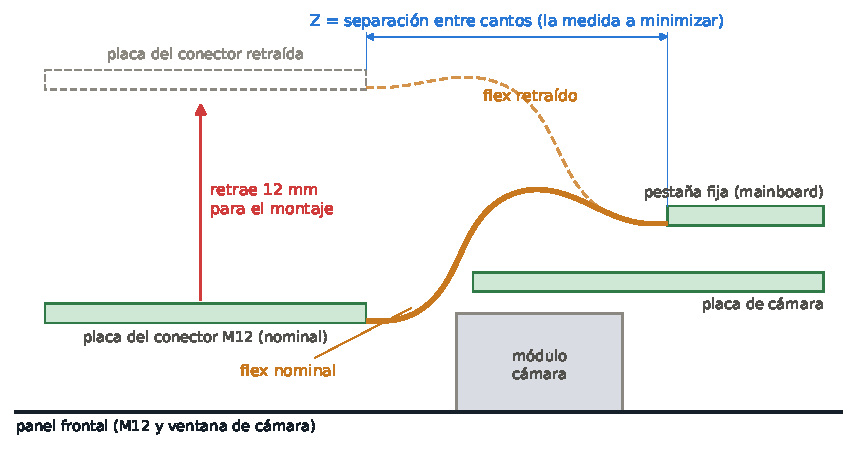
\includegraphics[width=0.72\linewidth]{fig_problema.pdf}
  \caption{Planta como en Solid Edge, con el panel abajo. Línea llena: flex en nominal; trazos: retraído
  12~mm. Esquema sobre el layout del 27/9.}
\end{figure}

\begin{table}[H]\centering\small
\caption{Condiciones de diseño.}
\begin{tabular}{l l >{\raggedright\arraybackslash}p{0.3\linewidth}}
\toprule
Condición & Valor & Origen\\
\midrule
Flex & 0,2~mm, 2 capas, 11~mm de alto & 48~V / 10~A y Ethernet\\
Radio interior mínimo & 2,5~mm & 12 veces el espesor (IPC-2223, 2 capas)\\
Recto en cada transición & 1~mm & regla de fabricación\\
Carrera & 12~mm (se verifica con 12,5) & montaje a través del panel\\
Altura disponible en nominal & 12 $-$ 0,1 = 11,9~mm & con cinta de 0,25~mm\\
Envolvente lateral & 52~mm, con la cámara y el LED & mecánica del equipo\\
Cantidad de flex & uno solo & fabricante (PCBWay)\\
Cuerpo del conector & 6,3 a 7~mm & tolerancia $\pm$0,35~mm\\
\bottomrule
\end{tabular}
\end{table}

\section{Cómo llegamos acá}
Cada propuesta respondió a una limitación de la anterior. W es el ancho total en el sentido de la
carrera; Z, la separación entre cantos de la S. La sección~\ref{sec:alternativas} muestra cada una
en imagen.

\begin{table}[H]\centering\footnotesize\setlength{\tabcolsep}{4pt}\renewcommand{\arraystretch}{1.1}
\begin{tabular}{r >{\raggedright\arraybackslash}p{0.33\linewidth} >{\raggedright\arraybackslash}p{0.24\linewidth} >{\raggedright\arraybackslash}p{0.30\linewidth}}
\toprule
\# & Propuesta & Resultado & Decisión\\
\midrule
1 & Omega en el plano vertical, placa del conector colgando (9,5~$-$~R) & W $\approx$ 32~mm; con R~3 no entra en la altura & buscar algo más angosto\\
2 & Omega del primer boceto & W = 26,4~mm, R~2,7 & admitir R~2,5: W = 25,7~mm\\
3 & Placa del conector en el piso, flex hacia arriba & W $\approx$ 24~mm & sigue ancho: pensar el flex en 3D\\
4 & \textbf{S de canto, en el plano de las placas} & W $\approx$ 13~mm & \textbf{camino elegido}\\
5 & U rodante & pide un canal libre de 7,6~mm & descartada\\
6 & Cámara con imagen horizontal & dobla demasiado el flex de la cámara & cámara centrada, flex recto, imagen a 90°\\
7 & Cámara + S doble, islas de flex & dos brazos de flex en una pieza & no fabricable: un solo flex\\
8 & LED junto al lente, sin guía de luz & variantes A, B y C & placa LED con conector B2B\\
9 & Dimensionar la S & Z 15,5 con R~3; Z 14 con R~2,5; pestaña 5~mm atrás & base del layout final\\
10 & \textbf{Layout del 27/9} con la placa de cámara como obstáculo & Z = 15,5; L = 19,0~$\pm$~0,25 & \textbf{solución de esta nota}\\
\bottomrule
\end{tabular}
\end{table}

\section{Geometría}\label{sec:geometria}
Coordenadas en mm, en planta y en posición nominal: \textbf{z} hacia la derecha desde el extremo izquierdo
de la placa del conector; \textbf{x} hacia el panel desde la línea del flex en la placa del conector
($x = 0$). El flex sale por la cara delantera de las dos placas.

\begin{table}[H]\centering\small
\begin{tabular}{l r r}
\toprule
Referencia & z & x\\
\midrule
Canto de la placa del conector (salida del flex) & 16,50 & 0,00\\
Canto de la pestaña fija (salida del flex) & 32,00 & $-$5,00\\
Cara trasera de la placa de cámara & desde 22,0 & $-$2,50\\
Inicio del módulo de cámara & 21,16 & ---\\
\bottomrule
\end{tabular}
\end{table}

\subsection{Geometría para dibujar}
La forma real tiene radios variables. Para el modelo 3D alcanza con tres arcos del mismo radio,
\textbf{R~3,5 en la línea media} (R~interior 3,4), unidos por rectas, con los mismos extremos, las mismas
tangentes y el mismo largo. En el equipo el flex toma su forma natural; el dibujo sirve para reservar el
espacio y obtener el largo desarrollado.

\begin{figure}[H]\centering
  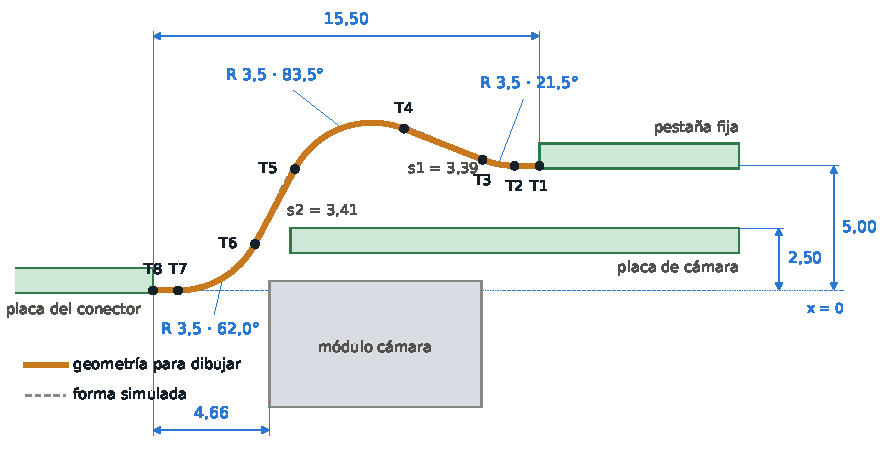
\includegraphics[width=\linewidth]{fig_geometria.pdf}
  \caption{Perfil para dibujar en nominal. En gris de trazos, la forma simulada: se aparta 0,11~mm como
  máximo del perfil de dibujo.}
\end{figure}

\begin{table}[H]\centering\small\setlength{\tabcolsep}{5pt}
\caption{Recorrido desde la pestaña fija (T1) hasta la placa del conector (T8).}
\begin{tabular}{l l l l r r}
\toprule
Tramo & Elemento & Medida & Gira hacia & Punto final (z; x) & Centro (z; x)\\
\midrule
T1--T2 & recta & 1,00 & --- & 31,000; $-$5,000 & ---\\
T2--T3 & arco & R~3,5 · 21,5° & atrás (lejos del panel) & 29,717; $-$5,244 & 31,000; $-$8,500\\
T3--T4 & recta & 3,39 & --- & 26,566; $-$6,485 & ---\\
T4--T5 & arco & R~3,5 · 83,5° & el panel & 22,193; $-$4,871 & 25,284; $-$3,228\\
T5--T6 & recta & 3,41 & --- & 20,590; $-$1,857 & ---\\
T6--T7 & arco & R~3,5 · 62,0° & atrás, hasta quedar paralelo & 17,500; 0,000 & 17,500; $-$3,500\\
T7--T8 & recta & 1,00 & --- & 16,500; 0,000 & ---\\
\midrule
 & \textbf{total} & \textbf{19,00} & & & \\
\bottomrule
\end{tabular}
\end{table}

Para trazarlo en Solid Edge:
\begin{enumerate}[leftmargin=1.6em]
  \item Croquis como cadena de rectas y arcos tangentes, con T1 en (32; $-$5) y T8 en (16,5; 0); en los
        dos extremos el flex sale paralelo a la placa.
  \item Acotar los tres radios en 3,5, las rectas de los extremos en 1,00 y los ángulos 21,5° y 62°.
        El arco central sale solo: 21,5 + 62 = 83,5°. Las rectas intermedias (3,39 y 3,41) también.
  \item Pestaña por contorno sobre el croquis: espesor 0,2, alto 11, factor neutro 0,5. El desarrollo
        da 19,00~mm.
\end{enumerate}

El juego del perfil de dibujo a la placa de cámara es 1,93~mm. Su radio interior es 3,4~mm, pero el
flex real llega a 2,84~mm: el radio se verifica con la simulación, no con el dibujo.

\subsection{Especificación para fabricar}
\begin{table}[H]\centering\small
\begin{tabular}{l l}
\toprule
Parámetro & Valor\\
\midrule
Largo del flex entre cantos rígidos & \textbf{19,0~$\pm$~0,25~mm}\\
Largo mínimo absoluto & 18,5~mm\\
Rectos en las transiciones & 1,0~mm en cada extremo\\
Espesor y capas & 0,2~mm, 2 capas\\
Alto del flex & 11~mm\\
Separación entre cantos (Z) & 15,5~mm\\
\bottomrule
\end{tabular}
\end{table}

El perfil exacto de la forma simulada (8 elementos, desvío 0,02~mm) queda como referencia en el plano
FX-M12-S-03 y en el DXF del perfil nominal, los dos en \texttt{flex\_omega/planos/}, y en
\texttt{resultados.json}.

\section{Verificación en la carrera}
\textbf{Método.} El flex se modela como una elástica: tira inextensible con los extremos empotrados que
adopta la forma de mínima energía de flexión; las paredes y la placa de cámara entran como obstáculos.
Se barre la carrera en los dos sentidos (nominal $\to$ retraído $\to$ nominal), arrancando desde
nominal, y se repite para el cuerpo del conector de 6,3 a 7~mm, la carrera de 12 y 12,5~mm y el
largo del flex $\pm$0,25~mm. Se informa siempre el peor resultado.

\begin{figure}[H]\centering
  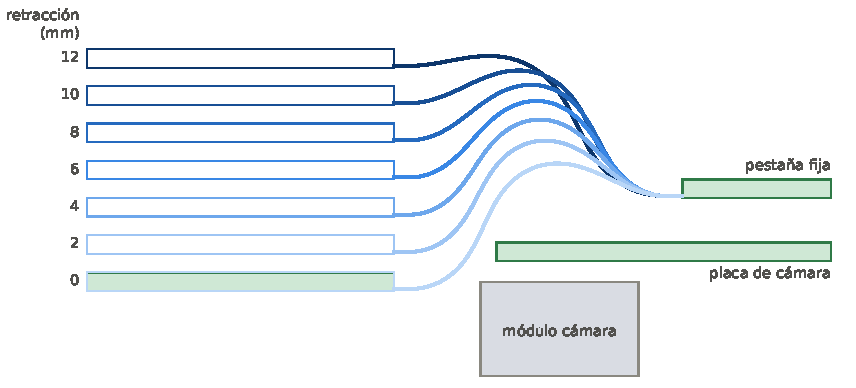
\includegraphics[width=0.7\linewidth]{fig_carrera.pdf}
  \caption{Forma del flex cada 2~mm de retracción, de 0 (nominal) a 12~mm. La S se abre hacia atrás y no
  toca la placa de cámara.}
\end{figure}

\begin{figure}[H]\centering
  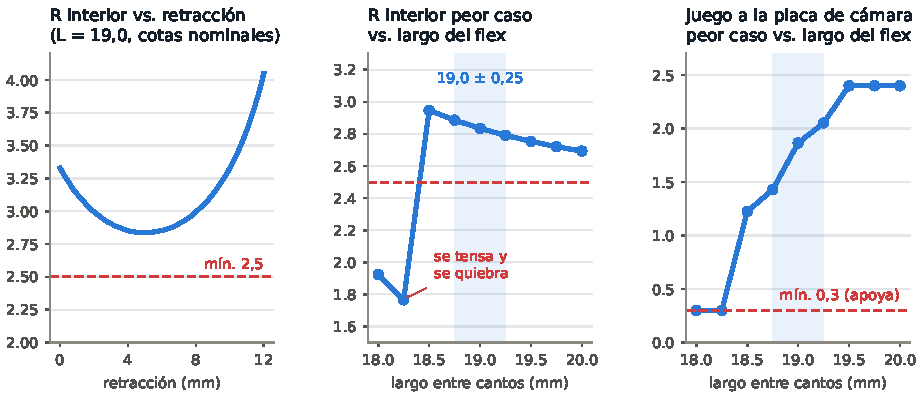
\includegraphics[width=0.82\linewidth]{fig_robustez.pdf}
  \caption{Izquierda: R interior en la carrera, con L = 19,0 y cotas nominales (mínimo 2,84~mm cerca de
  los 5~mm). Centro y derecha: peor caso de R interior y de juego según el largo del flex; la banda es
  19,0~$\pm$~0,25.}
\end{figure}

\begin{table}[H]\centering\small
\begin{tabular}{r r r l}
\toprule
Largo (mm) & R interior (mm) & Juego (mm) & Veredicto\\
\midrule
18,25 & 1,77 & 0,30 & no: se tensa y apoya\\
18,50 & 2,95 & 1,22 & borde, sin margen para la tolerancia\\
\textbf{18,75} & 2,89 & \textbf{1,43} & sí (tolerancia $-$)\\
\textbf{19,00} & 2,84 & 1,87 & sí (nominal)\\
\textbf{19,25} & \textbf{2,79} & 2,05 & sí (tolerancia +)\\
20,00 & 2,69 & 2,40 & sí, pero ocupa más\\
\bottomrule
\end{tabular}
\end{table}

\textbf{Limitaciones}
\begin{itemize}
  \item \textbf{Cotas del layout:} se tomó la cota de 2,5~mm como la distancia de la cara trasera de la
        placa de cámara a la línea del flex del conector; la placa de cámara empieza en z $\approx$ 22 y el
        módulo, 4,66~mm después del canto de la placa del conector. Si cambian, se corre de nuevo
        \texttt{s\_layout.py} y \texttt{calculo.py}.
  \item \textbf{Rigidez uniforme:} el cobre de las dos capas cambia la rigidez local, no el largo ni la
        forma general.
  \item \textbf{Juego exigido:} 0,3~mm a la placa de cámara, criterio propio.
\end{itemize}

\section{Alternativas evaluadas}\label{sec:alternativas}
Una imagen por propuesta, con su resultado en una línea. La marca verde indica que la idea quedó, total
o parcialmente, en la solución.

\begin{figure}[H]\centering
  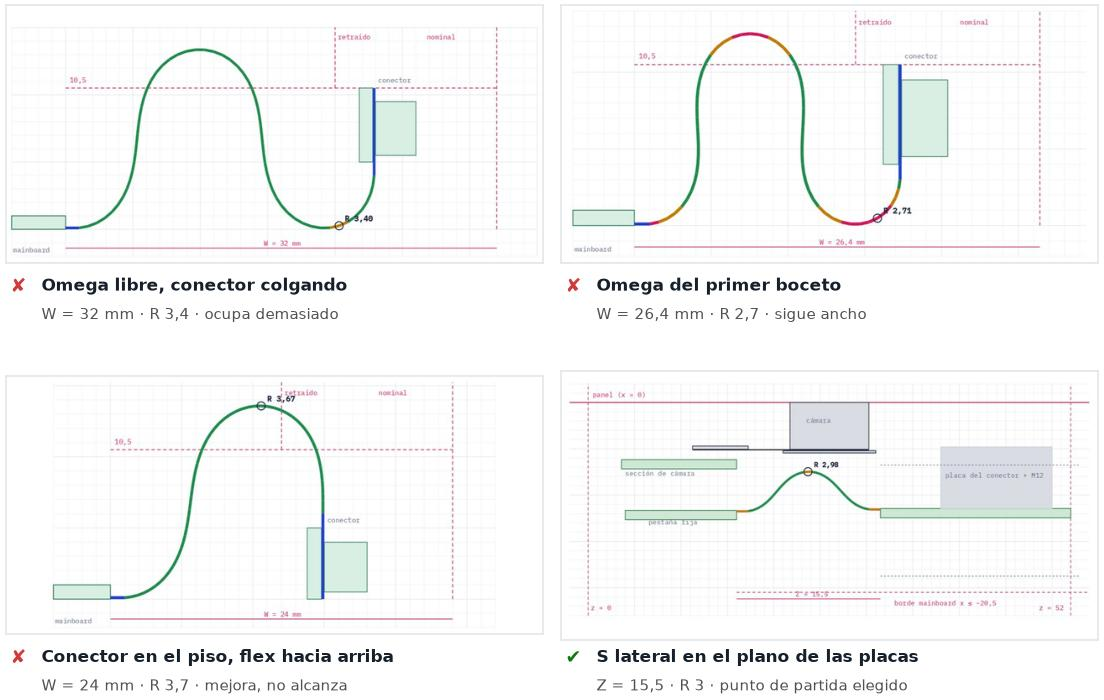
\includegraphics[width=\linewidth]{fig_galeria_1.jpg}
  \caption{Formas en el plano vertical (omega) y primera S en el plano de las placas.}
\end{figure}

\begin{figure}[H]\centering
  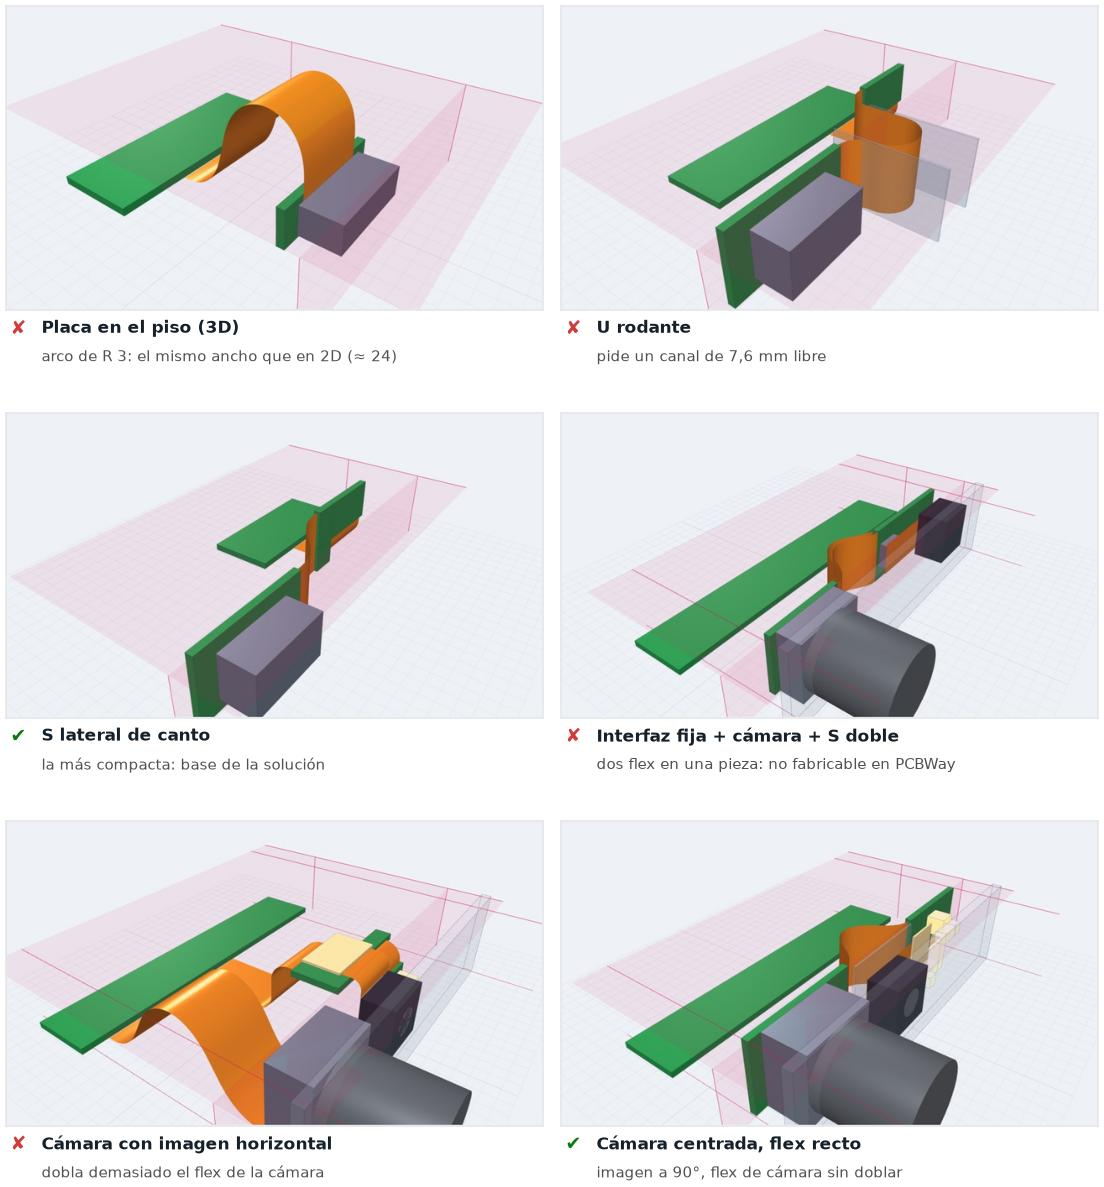
\includegraphics[width=0.93\linewidth]{fig_galeria_2.jpg}
  \caption{Arquitecturas en 3D e integración de la cámara.}
\end{figure}

\begin{figure}[H]\centering
  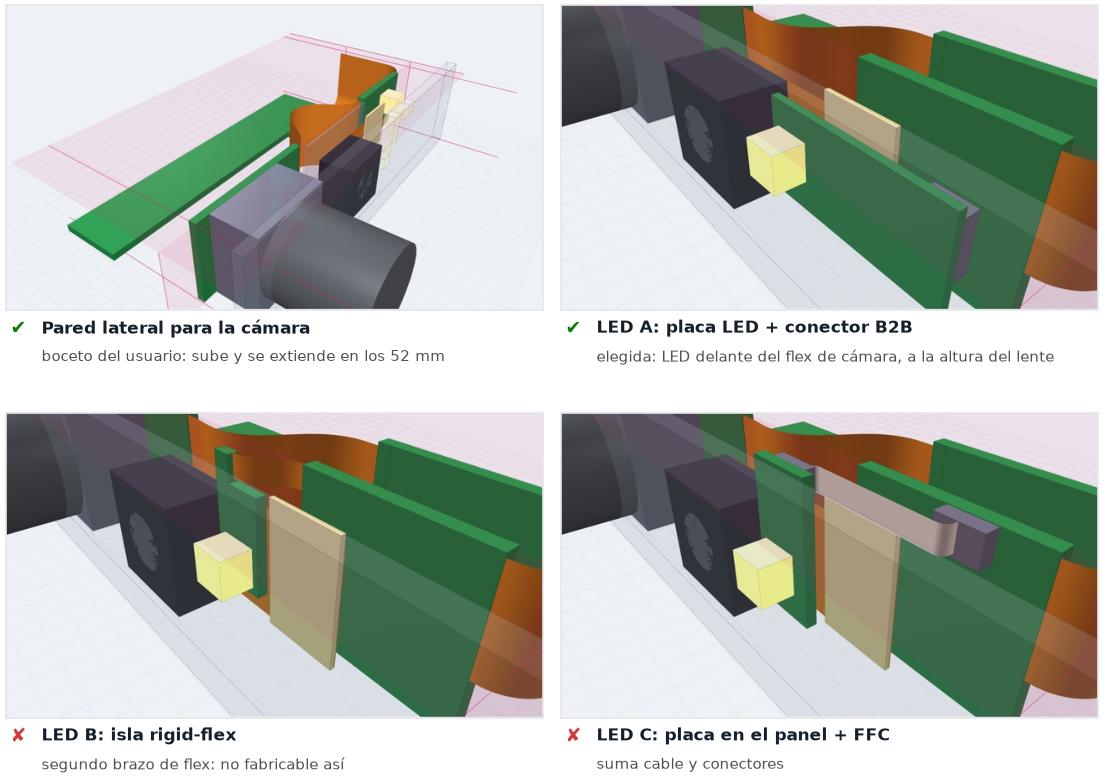
\includegraphics[width=\linewidth]{fig_galeria_3.jpg}
  \caption{Cámara en la pared lateral y variantes del LED.}
\end{figure}

\end{document}
